\chapter{Implementácia}
\label{kap:prakticka_cast}

V tejto kapitole podrobne popíšeme implementáciu autonómneho agenta pre hru Trackmania, vrátane použitých nástrojov, algoritmov a metód. Cieľom je vytvoriť systém, ktorý dokáže samostatne prechádzať pretekárske trate bez potreby ľudského zásahu. 

\section{Export 3D modelov blokov}

Modely hry Trackmania nie sú verejne dostupné v štandardných súboroch. Aby sme sa dostali ku geometrickým dátam o blokoch, najskôr sme pomocou projektu \cite{gbx_py_github} exportovali 3D mesh blokov z hry Trackmania. Tento nástroj nám umožnil dekódovať binárne súbory hry a extrahovať základné bloky, ktoré sme uložili do .obj súborov. Údaje ukladáme na pevný disk kvôli efektivite, keďže bloky stačí extrahovať iba jedenkrát. Tieto súbory obsahujú geometrické údaje o jednotlivých blokoch, ktoré sme následne použili na vytvorenie virtuálneho prostredia.

\begin{figure}
\centering
{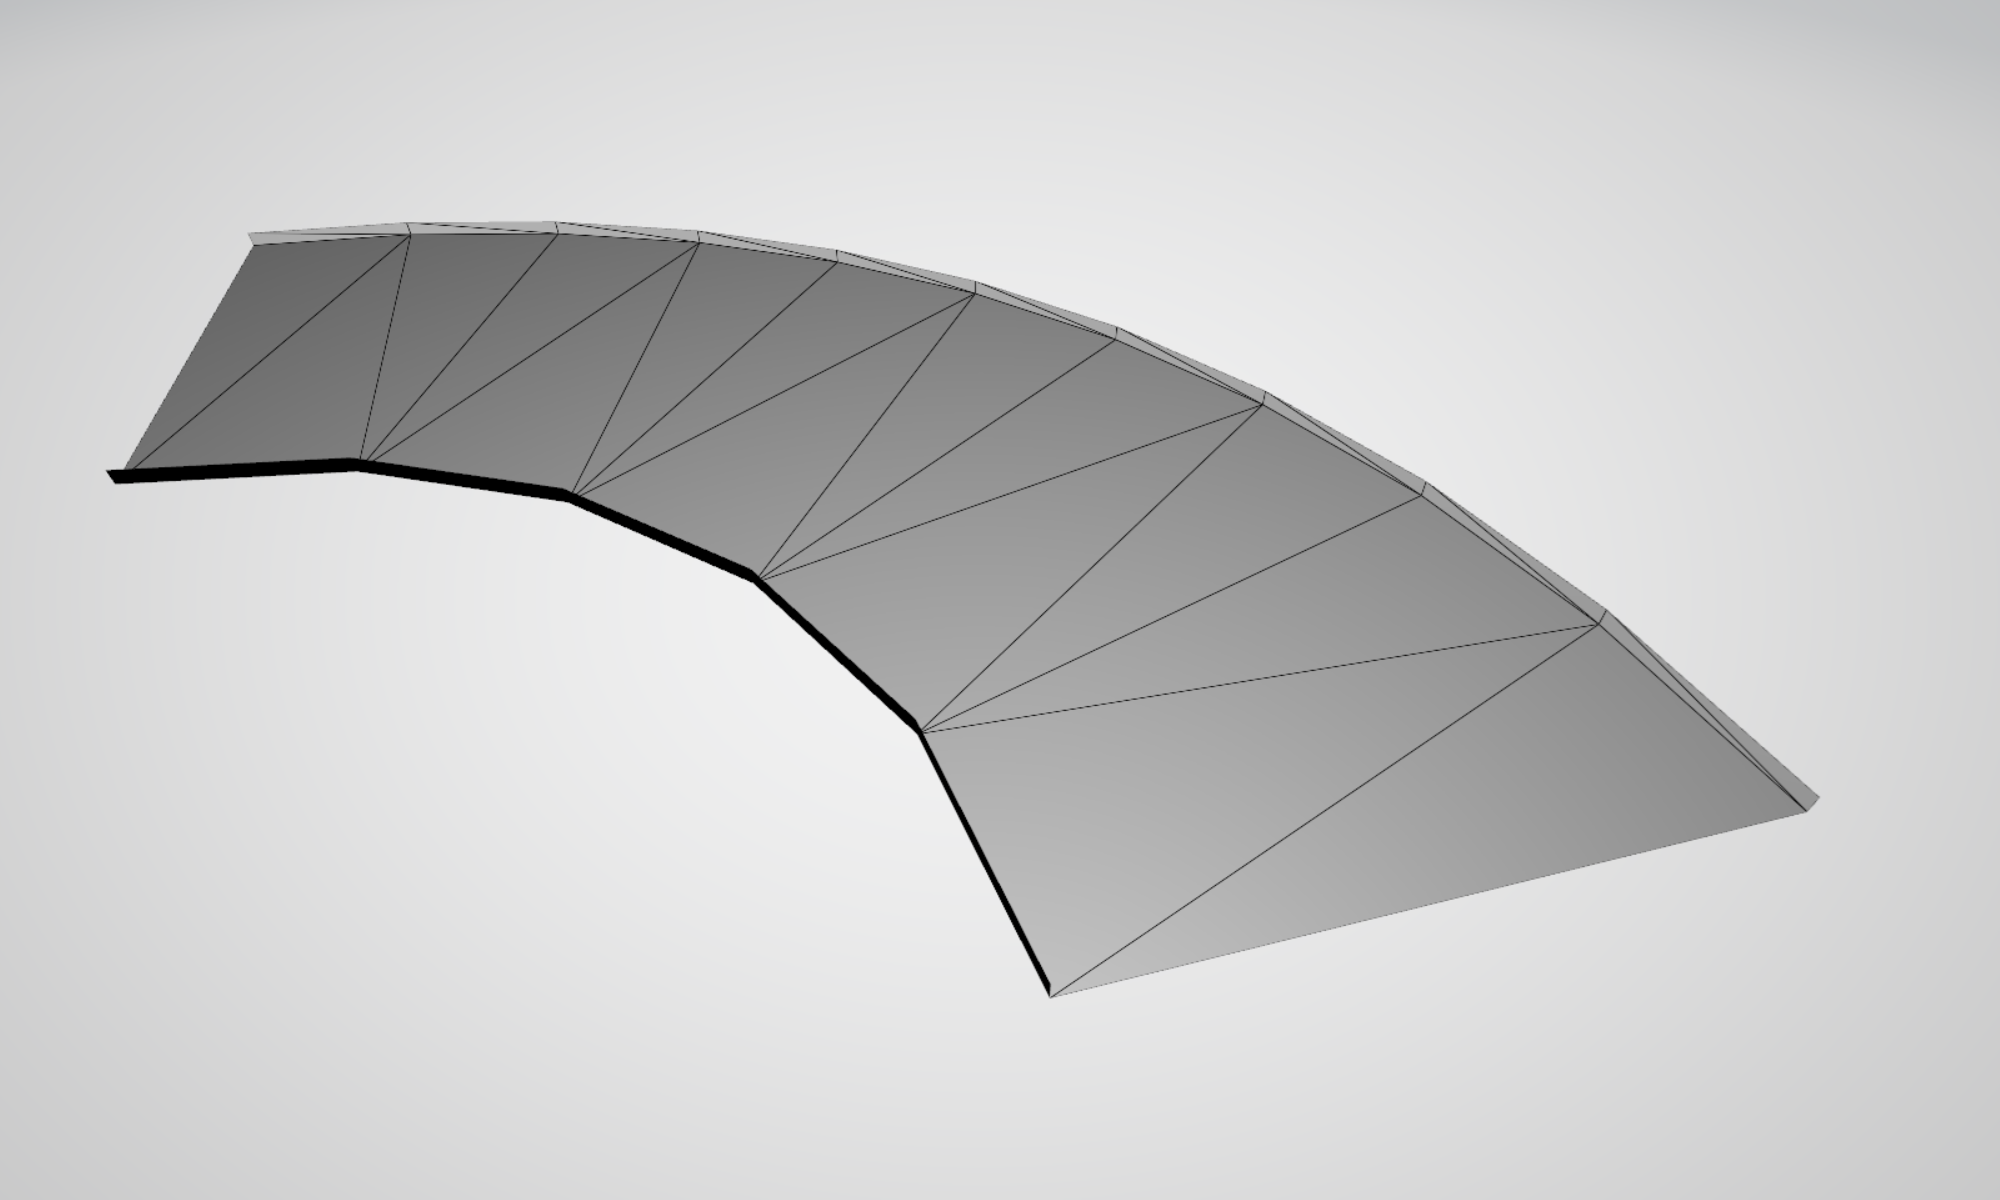
\includegraphics[width=0.45\textwidth]{images/mesh_curve.png}}
{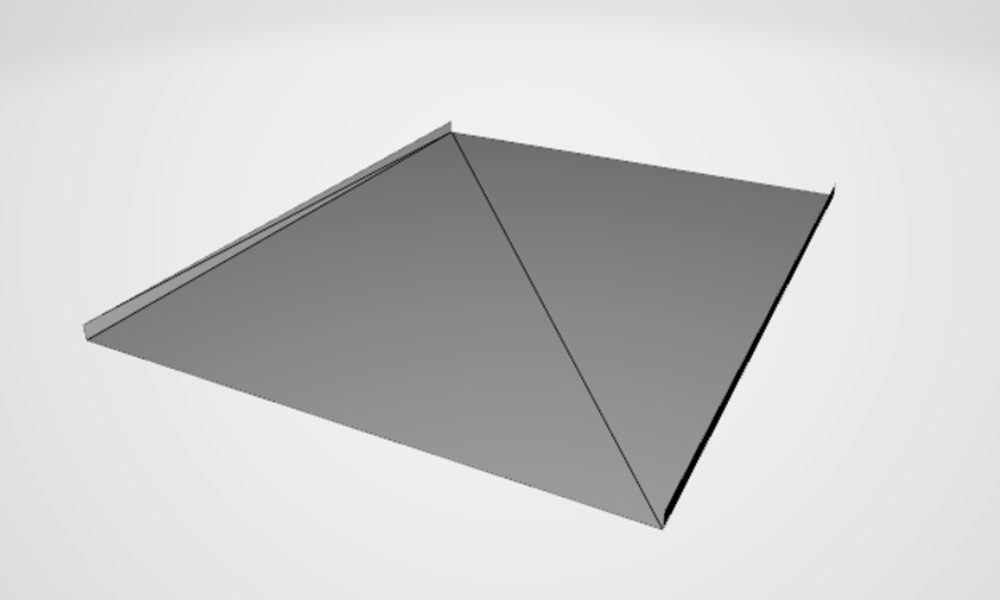
\includegraphics[width=0.45\textwidth]{images/mesh_straight.png}}
\caption[3D model blokov]{Na obrázku je znázornený blok zákruty a roviny, ktoré boli exportované do súboru s príponou .obj.}
\label{obr:block_mesh}
\end{figure}

\section{Extrahovanie údajov o mape}

Mapy Trackmanie sú uložené v binárnom súbore s príponou .gbx. Aby sme údaje z tohto binárneho súboru extrahovali, použili sme knižnicu GBX.NET, ktorá je implementovaná v jazyku C\#. Tento nástroj nám umožnil prechádzať jednotlivé bloky na mape a ukladať informácie o ich pozícii, type a otočení do textového súboru.

\begin{verbatim}
Pseudokód pre extrakciu údajov o blokoch:
1. Načítaj mapový súbor.
2. Vytvor nový textový súbor.
3. Pre každý blok v mape:
   a. Získaj pozíciu, typ a otočenie bloku.
   b. Zapíš pozíciu, typ, otočenie bloku na nový riadok.
\end{verbatim}

\section{Vytvorenie virtuálneho prostredia}

Pomocou knižnice \texttt{trimesh} v Pythone sme následne vytvorili 3D model trate. Každý blok sme umiestnili na správnu pozíciu a otočili podľa údajov získaných v predchádzajúcom kroku. Týmto spôsobom sme vytvorili virtuálne prostredie, kde môžeme simulovať LiDAR senzory pomocou raycastingu.

\begin{verbatim}
Pseudokód pre vytvorenie 3D modelu trate:
1. Načítaj údaje o blokoch z textového súboru.
2. Pre každý blok:
   a. Načítaj 3D model bloku (.obj súbor).
   b. Aplikuj transformácie (pozícia, otočenie).
   c. Pridaj blok do scény.
3. Vytvor a vráť 3D scénu.
\end{verbatim}

\begin{figure}
\centerline{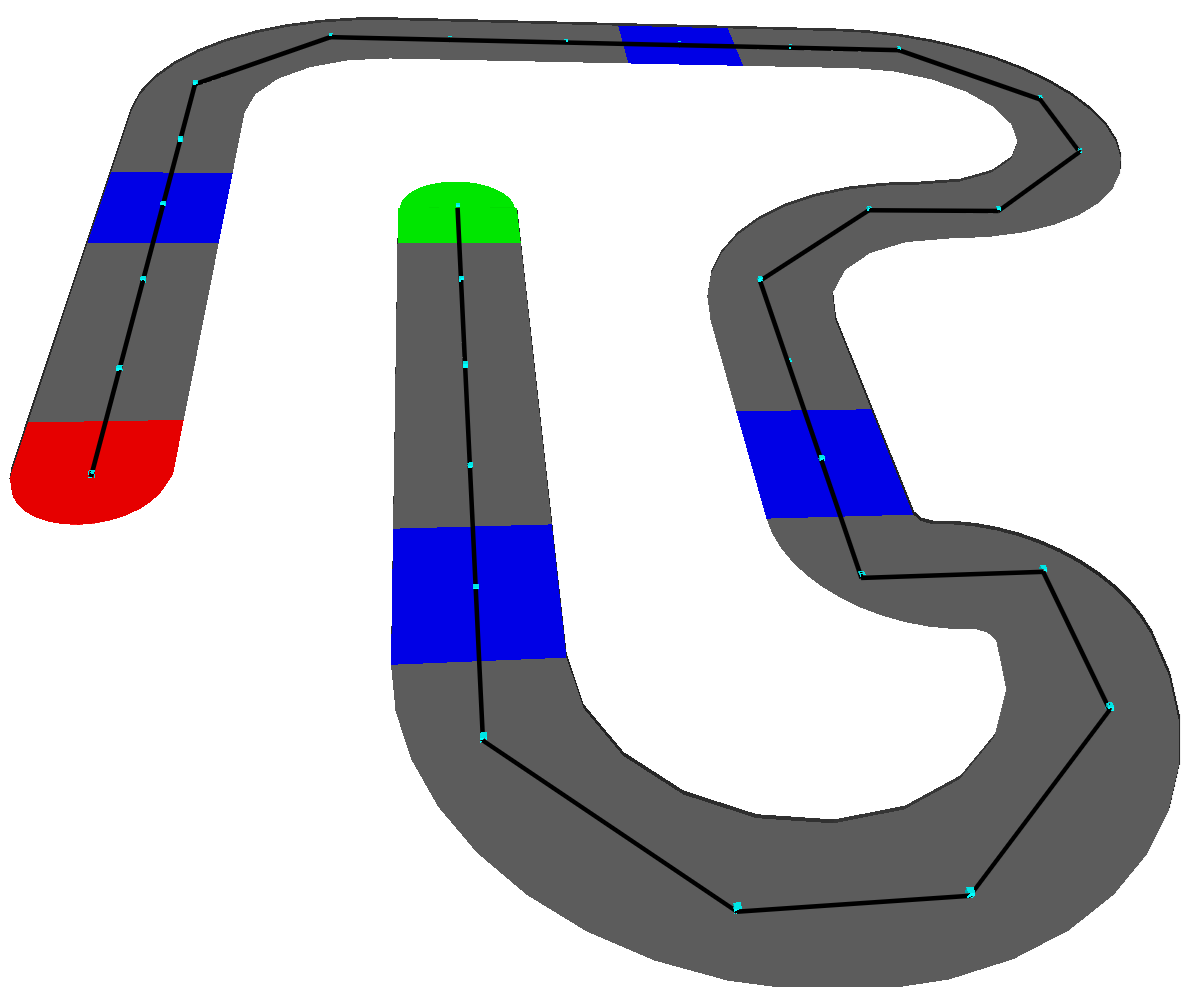
\includegraphics[width=0.65\textwidth]{images/virtual_track.png}}
\caption[Virtuálna mapa]{Na obrázku je zobrazený virtuálny model skutočnej mapy z Trackmanie. Tento model bol vyskladaný z 3D modelov stavebných blokov. Môžeme si všimnúť farebné zvýraznenie niektorých blokov, kde zelená farba znázorňuje štart, červená cieľ a modrá kontrolnú bránu.}
\label{obr:virtual_map}
\end{figure}

Na obrázku \ref{obr:virtual_map} si môžeme všimnúť, že blok sa skladá z dvoch hlavných častí: cesty a bariéry. Keďže sa nachádzame v jednej rovine, na detekciu prekážok nepotrebujeme poznať plochu cesty, preto scénu môžeme prefiltrovať o trojuholníky, ktorých normála má vertikálny smer.

\section{Získavanie dát o stave vozidla}

Na získavanie dát o stave vozidla sme použili plugin do OpenPlanet, ktorý je napísaný v jazyku AngelScript. Tento skript nadviaže TCP/IP spojenie na lokálnej úrovni a na každom snímku získa údaje o stave vozidla, ktoré následne pošle pomocou lokálneho spojenia.

\begin{verbatim}
Pseudokód pre získavanie dát o stave vozidla:
1. Nadviaž TCP/IP spojenie.
2. V nekonečnej slučke:
   a. Získaj údaje o stave vozidla
      (pozícia, rýchlosť, smer, otáčky motora).
   b. Pošli tieto údaje cez TCP/IP spojenie.
   c. Počkaj na ďalší snímok.
\end{verbatim}

\section{Simulácia LiDAR senzorov}

Trieda \texttt{Car} v Pythone uchováva aktuálne dáta o stave vozidla. Táto trieda obsahuje vlákno, ktoré udržiava TCP/IP spojenie s pluginom a neustále aktualizuje stav vozidla. Tento modul sa stará o samotné vysielanie lúčov a simulovanie LiDAR senzorov.

\begin{verbatim}
Pseudokód pre simuláciu LiDAR senzorov:
1. Inicializuj TCP/IP spojenie s hrou.
2. V nekonečnej slučke:
   a. Prijímaj údaje o stave vozidla cez TCP/IP spojenie.
   b. Vysielaj lúče z pozície auta rôznymi smermi.
   c. Aktualizuj stav vozidla.
\end{verbatim}


\begin{figure}
\centering
{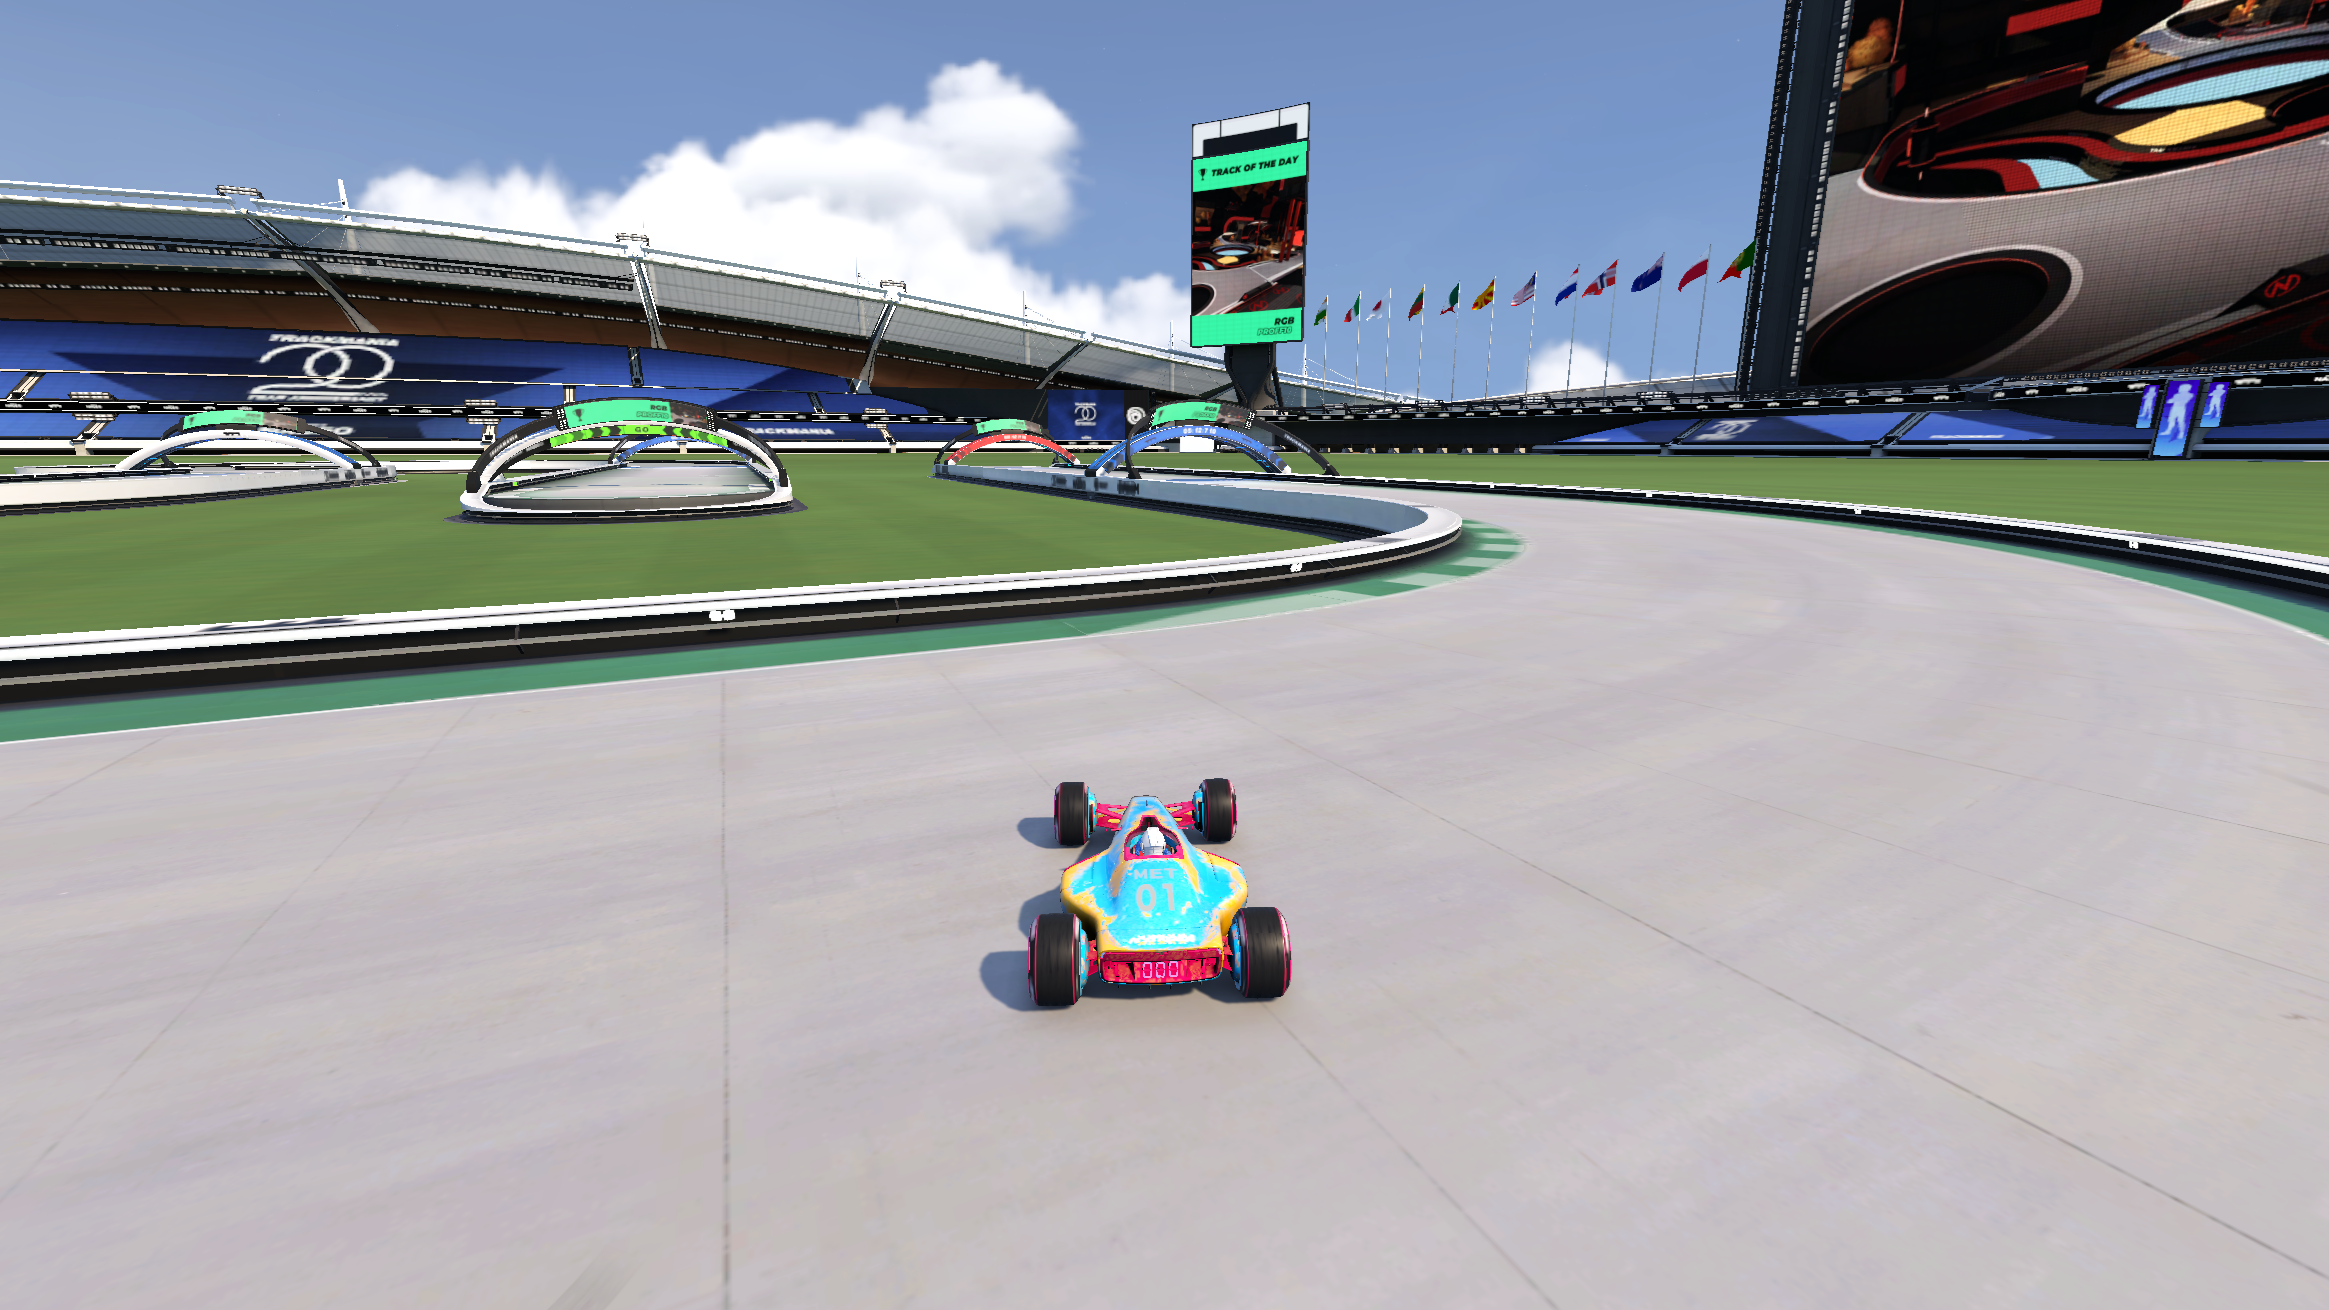
\includegraphics[width=0.45\textwidth]{images/game_view.png}}
{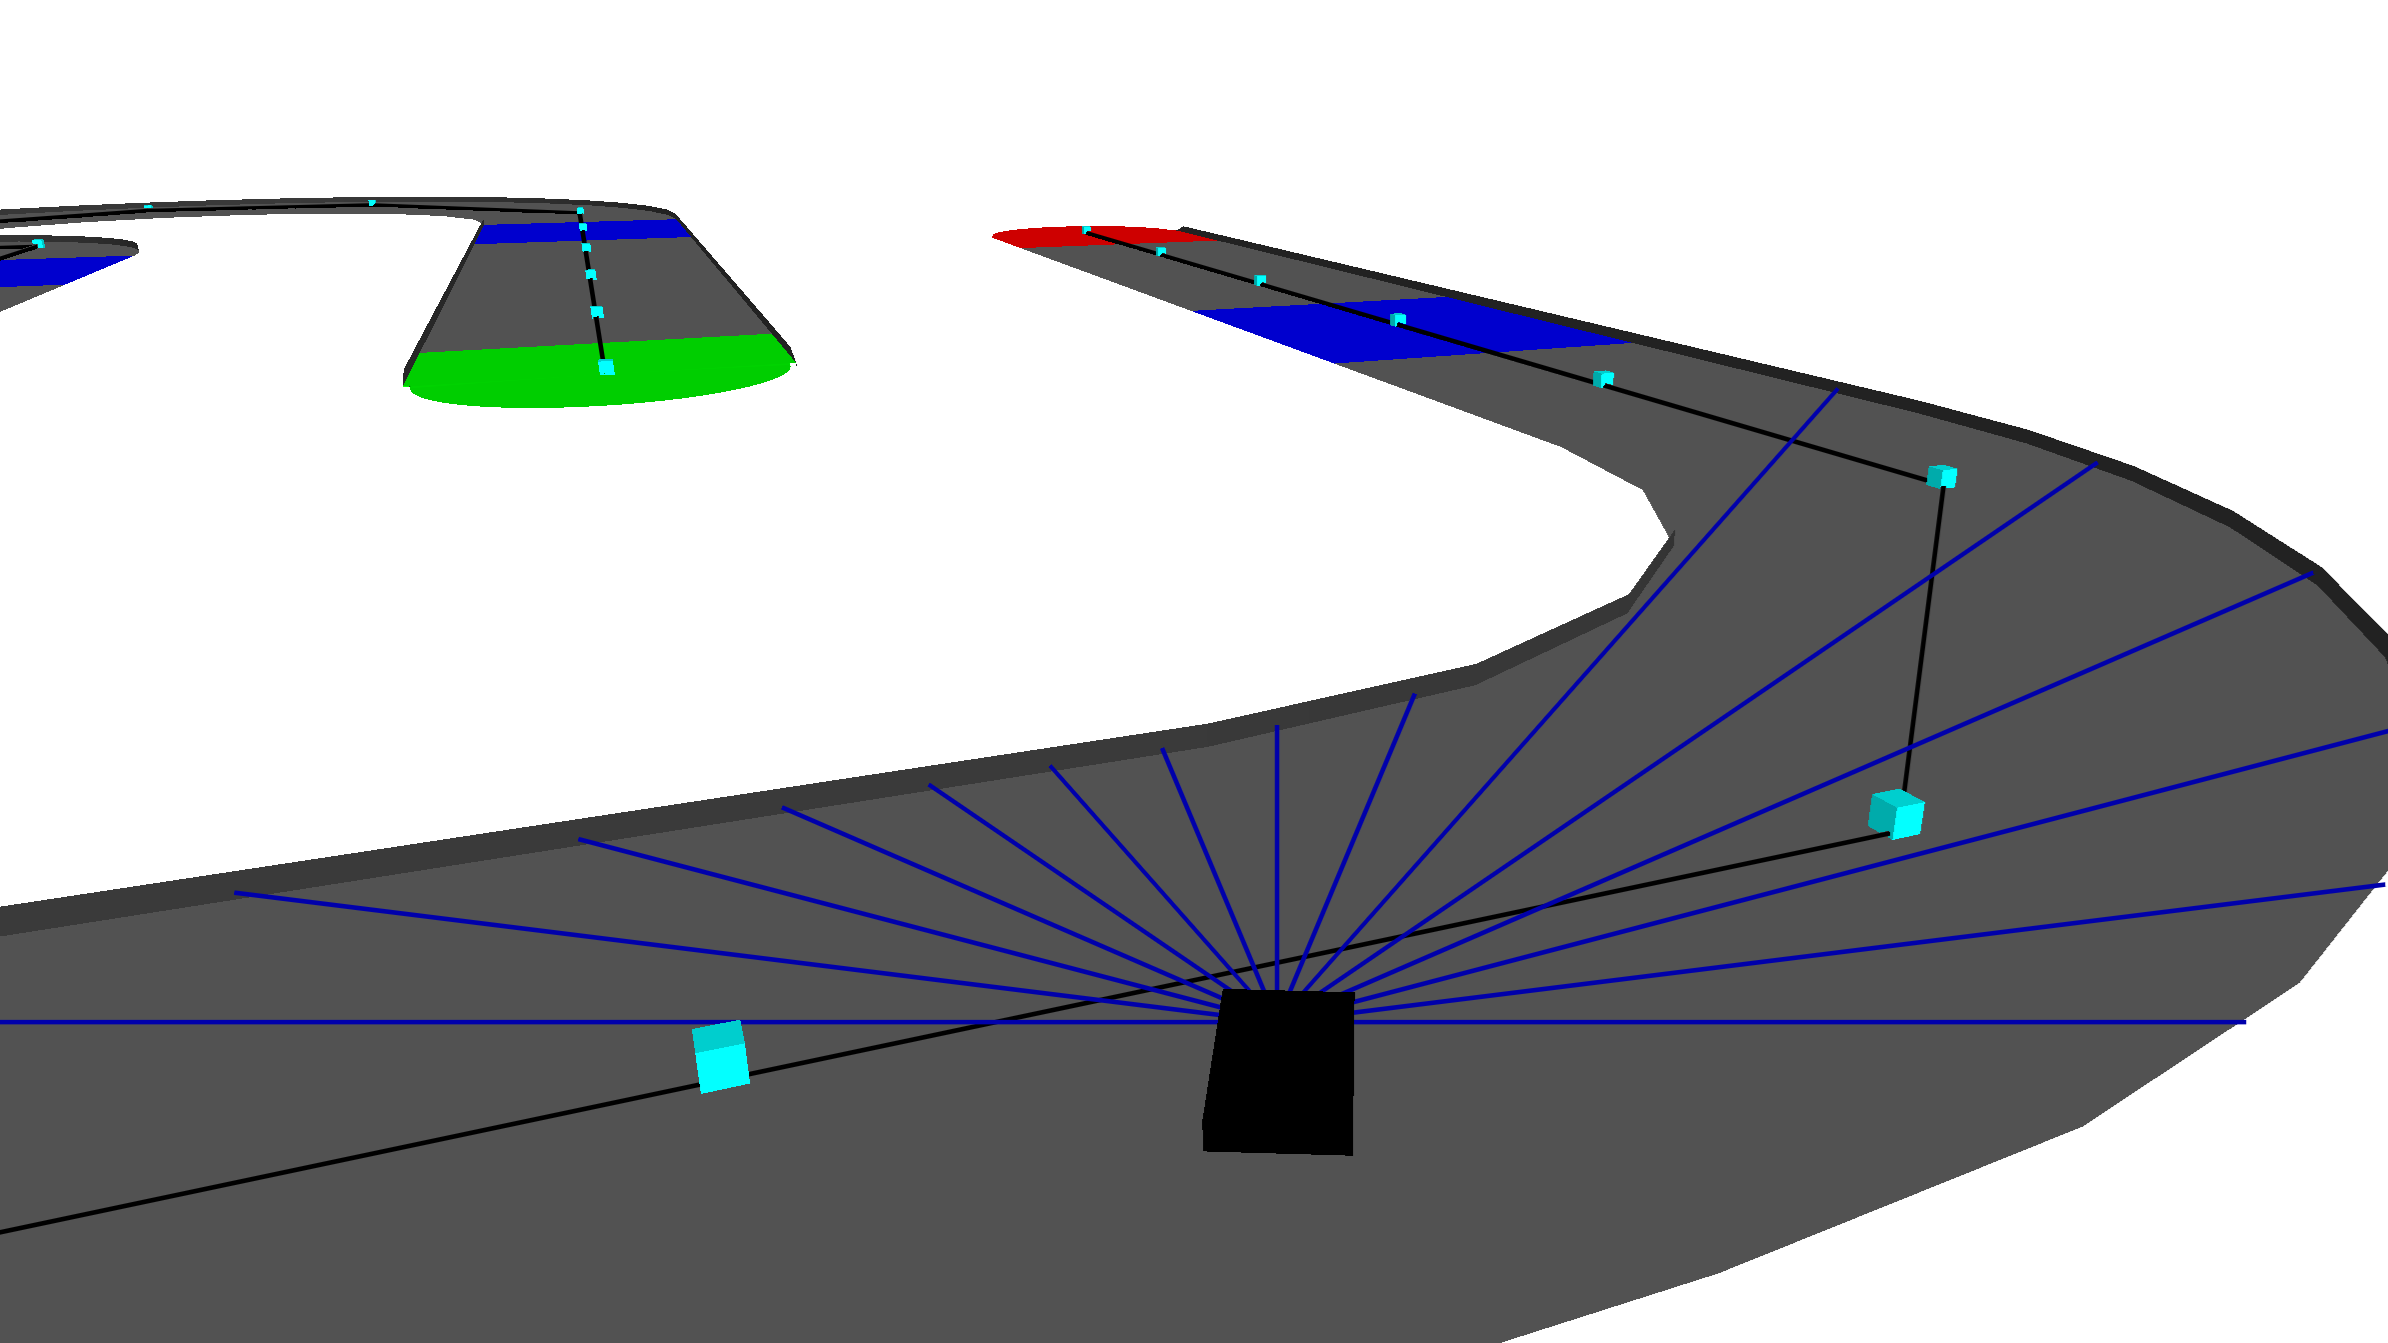
\includegraphics[width=0.45\textwidth]{images/agent_view.png}}
\caption[Pohľad agenta na hru]{Na obrázku môžeme vidieť simuláciu LiDAR senzora na nami vytvorenej kópii mapy. Takto môžeme vizuálne porovnať, ako náš agent vníma hru oproti jej skutočnej podobe.}

\label{obr:agent_vs_real}
\end{figure}


\section{Definícia prostredia}

Modul \texttt{Environment} integruje triedy \texttt{Car} a \texttt{Map} a definuje akcie vozidla pomocou virtuálneho analógového ovládača knižnice \texttt{vgamepad}. Náš modul \texttt{Environment} je obalený v triede \texttt{gym.Env}, čo nám umožňuje používať štandardné funkcie na trénovanie pomocou učenia posilňovaním v rôznych knižniciach.

\begin{verbatim}
Pseudokód pre definíciu prostredia:
1. Inicializuj triedy Car a Map.
2. Definuj akčné a pozorovacie priestory.
reset():
   a. Resetuj stav vozidla na štartovaciu pozíciu.
   b. Vráť počiatočný stav prostredia.
step(action):
   a. Aplikuj akciu na vozidlo.
   b. Aktualizuj stav hry.
   c. Vypočítaj odmenu.
   d. Skontroluj, či epizóda skončila.
   e. Vráť nový stav, odmenu, príznak ukončenia a dodatočné informácie.
\end{verbatim}

\section{Trénovanie agenta}

Na trénovanie agenta sme použili knižnicu \texttt{stable-baselines3}\cite{stable_baselines3}, ktorá poskytuje množstvo algoritmov na trénovanie. Vzhľadom na to, že sa pohybujeme v spojitom priestore, rozhodli sme sa použiť algoritmus Proximal Policy Optimization (PPO). Trénovanie agenta často trvalo desiatky hodín a preto bola každá malá zmena veľmi časovo nákladná.
\newline

\begin{verbatim}
Pseudokód pre trénovanie agenta:
1. Vytvor environment pomocou TrackmaniaEnv
2. Inicializuj model PPO s príslušnou politikou
3. Trénuj model s daným počtom časových krokov
4. Ulož natrénovaný model
\end{verbatim}

Samotné trénovanie agenta prebiehalo na trati, ktorú môžeme vidieť na obrázku \ref{obr:training_map}. Táto trať obsahuje dostatočné množstvo rozmanitých zákrut, čím sa vyhneme pretrénovaniu agenta na určitú postupnosť zákrut. Trénovanie agenta sme rozdelili do troch fáz, podľa toho, akú odmeňovaciu funkciu sme použili:

\begin{enumerate}
    \item Agent dostal odmenu za pohyb vpred v smere trate a za stláčanie klávesy plynu. Týmto sme dosiahli, že agent nezostal stáť na mieste, ale pokúsil sa o pohyb vpred, aj keď zo začiatku často havaroval.
    \item Keď bol agent schopný pohybu vpred, zmenili sme funkciu tak, aby agent stále dostával pozitívnu odmenu za progresovanie na trati, ale zároveň dostal negatívnu odmenu za kolíziu s bariérou trate alebo za bezprostredné priblíženie sa k nej. Týmto prístupom sme donútili agenta aby nebúral a neustále postupoval po mape, aj keď možno pomalým tempom.
    \item Ak agent dokázal konzistentne prejsť celú trať až do cieľa, zmenili sme finálnu odmenu iba s ohľadom na záporný výsledný čas agenta. Keďže sa agent snaží odmenu maximalizovať, bude odmenený za čo najkratší čas prejdenia trate.
\end{enumerate}

Okrem odmeňovacej funkcie sme experimentovali aj s počtom vysielaných lúčov, aby sme našli rovnováhu medzi rýchlou odozvou a dostatočnosťou informácií o okolí. Taktiež sme skúšali rôzne hodnoty pre rýchlosť trénovania, ktorá ovplyvňuje intenzitu úpravy váh v neurónovej sieti. Príliš rýchle trénovanie môže viesť k neoptimálnemu riešeniu a uviaznutiu v lokálnom minime. Príliš pomalé trénovanie zase spôsobuje pomalý pokrok a takéto trénovanie býva častokrát časovo náročnejšie. Knižnica \texttt{stable-baselines3} nám väčšinu technických aspektov, ako štruktúra skrytej vrstvy neurónovej siete alebo algoritmy trénovania, vyriešila za nás.

\begin{figure}
\centerline{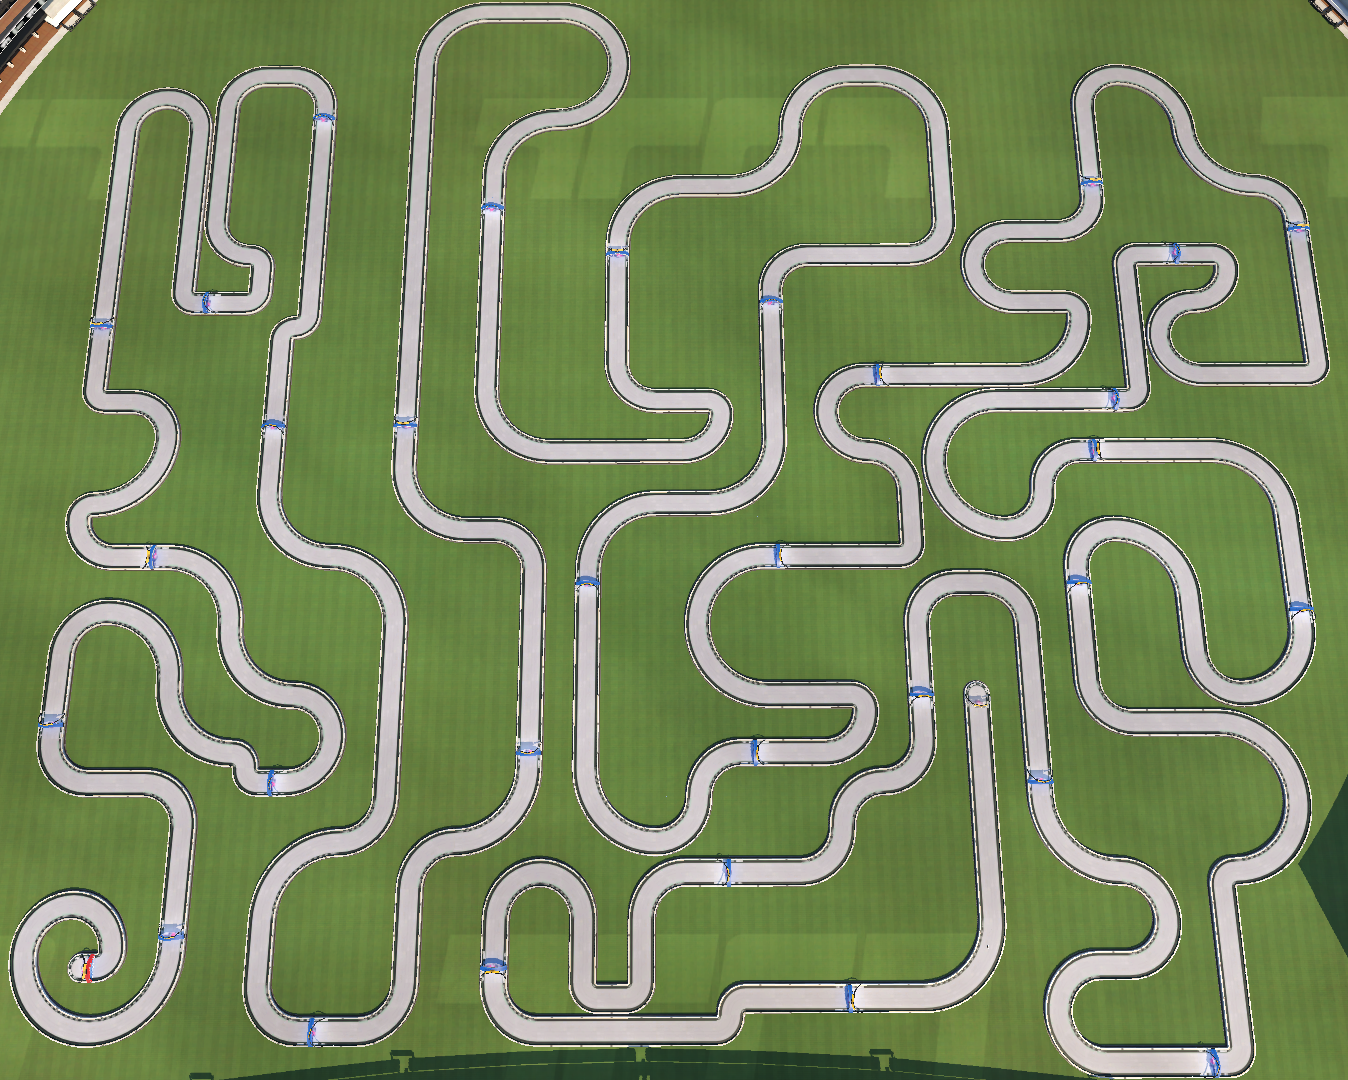
\includegraphics[width=0.65\textwidth]{images/training_map.png}}
\caption[Trénovacia mapa]{Na obrázku je zobrazený pôdorys tréningovej mapy, ktorá bola vytvorená, aby obsahovala čo najrozmanitejšie typy zákrut. Táto trať je tvorená výlučne asfaltovými blokmi a jej úspešné prejdenie vyžaduje približne 4 minúty jazdy.}
\label{obr:training_map}
\end{figure}

\section{Používanie natrénovaného modelu}

Modul \texttt{Driver} načíta natrénovaný model a podľa neho vykonáva požadované akcie. Tento modul zabezpečuje to, aby agent vedel správne interagovať s herným prostredím na základe predikcií modelu.
\newline
\begin{verbatim}
Pseudokód pre používanie natrénovaného modelu:
1. Načítaj natrénovaný model
2. Inicializuj environment
3. V nekonečnej slučke:
   a. Získaj aktuálny stav prostredia
   b. Predikuj akciu pomocou modelu
   c. Aplikuj akciu na vozidlo
   d. Aktualizuj stav hry
\end{verbatim}

